   %\title{LaTeX Portrait Poster Template}
%%%%%%%%%%%%%%%%%%%%%%%%%%%%%%%%%%%%%%%%%
% a0poster Portrait Poster
% LaTeX Template
% Version 1.0 (22/06/13)
%
% The a0poster class was created by:
% Gerlinde Kettl and Matthias Weiser (tex@kettl.de)
% 
% This template has been downloaded from:
% http://www.LaTeXTemplates.com
%
% License:
% CC BY-NC-SA 3.0 (http://creativecommons.org/licenses/by-nc-sa/3.0/)
%
%%%%%%%%%%%%%%%%%%%%%%%%%%%%%%%%%%%%%%%%%

%----------------------------------------------------------------------------------------
%   PACKAGES AND OTHER DOCUMENT CONFIGURATIONS
%----------------------------------------------------------------------------------------

\documentclass[a0,portrait]{a0poster}

\usepackage{multicol} % This is so we can have multiple columns of text side-by-side
\columnsep=100pt % This is the amount of white space between the columns in the poster
\columnseprule=3pt % This is the thickness of the black line between the columns in the poster

\usepackage[svgnames]{xcolor} % Specify colors by their 'svgnames', for a full list of all colors available see here: http://www.latextemplates.com/svgnames-colors

\usepackage{times} % Use the times font
%\usepackage{palatino} % Uncomment to use the Palatino font

\usepackage{graphicx} % Required for including images
\graphicspath{{figures/}} % Location of the graphics files
\usepackage{booktabs} % Top and bottom rules for table
\usepackage[font=small,labelfont=bf]{caption} % Required for specifying captions to tables and figures
\usepackage{amsfonts, amsmath, amsthm, amssymb} % For math fonts, symbols and environments
\usepackage{wrapfig} % Allows wrapping text around tables and figures
\usepackage{arydshln}


%
% Chinese
%

\usepackage{xeCJK}
\setCJKmainfont{Noto Sans CJK TC Regular}

\XeTeXlinebreaklocale "zh"
\XeTeXlinebreakskip = 0pt plus 1pt

\makeatletter
\def\hlinewd#1{%
  \noalign{\ifnum0=`}\fi\hrule \@height #1 \futurelet
   \reserved@a\@xhline}
\makeatother


\graphicspath{{./figures/}} 


\begin{document}

%----------------------------------------------------------------------------------------
%   POSTER HEADER 
%----------------------------------------------------------------------------------------

% The header is divided into two boxes:
% The first is 75% wide and houses the title, subtitle, names, university/organization and contact information
% The second is 25% wide and houses a logo for your university/organization or a photo of you
% The widths of these boxes can be easily edited to accommodate your content as you see fit

\begin{minipage}[b]{0.75\linewidth}
\veryHuge \color{NavyBlue} \textbf{Game Playing with DQfD and DQN} \color{Black}\\ % Title
\Huge\textit{ADL Final Project}\\[2cm] % Subtitle
\huge \textbf{Team: Praise the Sun}\\[0.5cm] % Author(s)
\huge Department of Computer Science, National Taiwan University\\[0.4cm] % University/organization
%\Large \texttt{john@LaTeXTemplates.com} --- 1 (000) 111 1111\\
\end{minipage}
%
\begin{minipage}[b]{0.25\linewidth}

\includegraphics[width=12.5cm]{ntu_logo.png}\\
\end{minipage}

\vspace{1cm} % A bit of extra whitespace between the header and poster content

%----------------------------------------------------------------------------------------

\begin{multicols}{2} % This is how many columns your poster will be broken into, a portrait poster is generally split into 2 columns

%----------------------------------------------------------------------------------------
%   ABSTRACT
%----------------------------------------------------------------------------------------

\color{Navy} % Navy color for the abstract

\begin{abstract}

Deep reinforcement learning are learning models that combines traditional reinforcement learning algorithms with modern state-of-the-art deep learning models. Currently, many applications, such as robotics and game playing, have reached astonishing performances with these kinds of models. However, these models require huge amount of time/self-generated data to achieve favorable results. What worse is that the performances are sometimes even unstable: the results may differ even given the same environments and model settings. Some recent advanced algorithms may make the training process more efficient, for instance, the \emph{Deep Q-Learning from Demonstrations}(DQfD) proposed by (T. Hester et al., 2017)\cite{DBLP:journals/corr/HesterVPLSPSDOA17}, which introduced the so-called ``demonstration data'' that can train deep RL models in a supervised manner. In this project, we used some Atari games as the training environment, and we did some experiments on some traditional value-based deep reinforcement learning algorithms and on DQfD, and made some comparisons and analysis on our experiments.



\end{abstract}

%----------------------------------------------------------------------------------------
%   INTRODUCTION
%----------------------------------------------------------------------------------------

\color{DarkSlateGray} % DarkSlateGray color for the rest of the content

\section*{Background}
A reinforcement learning model contains an environment and an agent, in which the behavior of the agent can be modeled as a Markov decision process (MDP). MDP can be formally represented by a 5-tuple $(S,A,R(\cdot,\cdot),T(\cdot, \cdot, \cdot),\gamma)$, where $S$ denotes the set of states, $A$ represents the set of all possible actions, $R(s,a)$ is a reward function (given current state $s$ and action $a$, $R$ returns the reward), $T(s,a,s')=P(s'|s,a)$ is a transition function, which follows some distribution, and $\gamma$ is the discount factor. The agent can be regarded as being applying some policy function $\pi(s)$ in the environment to take actions.\par

The most common reinforcement learning models can be classified as \emph{policy-baced} and \emph{value-based}. The former tries to find a policy function $\pi$ such that it can be as close with the optimal policy as possible (i.e. $\pi \rightarrow \pi^*$), while the latter is to learn a value function $Q^\pi (s,a)$, whose objective is to estimate the expected value given the current state $s$ and action $a$, and we hope that the value function we are training can be as close to the optimal one as possible (i.e. $Q^\pi (s,a) \rightarrow Q^* (s,a)$). Under such circumstance, the optimal policy for the agent will be $\pi^*(s) = \arg \underset{a \in A}\max\ Q^*(s,a)$.\par

Deep Q Learning (DQN) is one of the most common value-based deep learning algorithms. Its optimal value function can be represented as a Bellman equation:
\[Q^*(s,a) = \mathbb{E}\left[R(s,a) + \gamma \sum_{s'}P(s'|s,a) \underset{a'}\max\ Q^*(s',a')\right]\]
In a DQN model, we'll use a neural network to represent $Q^\pi$,and we expect that $Q^\pi$ will eventually converge to $Q^*$. In practice, we often use mean squared error (MSE) as the loss function for training, and moreover, for stablility, we also stablize the weights of the target network, and the loss function is as follows:
\[\mathcal{L}(w) = \mathbb{E}\left[\left(\underbrace{R(s,a) + \gamma \underset{a'}\max\ Q(s',a', w^-)}_{\text{target, update slowly}} - \underbrace{Q(s,a,w)}_{\text{online, update quickly}}\right)^2\right]\]
\par
There are some other common DQN models, including Double Q-Learning(DDQN)(H. van Hasselt et al., 2015)\cite{DBLP:journals/corr/HasseltGS15}, Dueling Network (Z. Wang et al., 2015)\cite{DBLP:journals/corr/WangFL15}, etc. The former points out that upward bias may occurs when using target network to select the action that has the largest expected value, and thus the (new) loss function is as follows:
\[\mathcal{L}(w) = \mathbb{E}\left[\left(R(s,a) + \gamma Q(s',\underbrace{\arg \underset{a'}\max\ Q(s',a',w)}_{\text{online network chooses optimal } a'}, w^-) - Q(s,a,w)\right)^2\right]\], while the latter modifies the network as:
\[Q(s,a,w) = \underbrace{V(s,w)}_{\text{\emph{value}, action-independent}} + \underbrace{A(s,a,w)}_{\text{\emph{advantage}, action-dependent}}\]
The basic idea is that some states are just better (regardless of the actions taken), while others not. Hence the expected value can be cosidered to be the sum of the expected value of the state (action-independent) and the added/subtracted value given a certain action.

%----------------------------------------------------------------------------------------
%   OBJECTIVES
%----------------------------------------------------------------------------------------

%\color{SaddleBrown} % SaddleBrown color for the introduction


\section*{DQfD:Learning from Demonstrated Data}


\textbf{Deep Q-Learning from Demonstrations} (DQfD) is a kind of deep reinforcement learning algorithm that contains elements of supervised learning. Unlike the original DQN, DQfD will perform pre-training on some pre-collected demonstration data prior to the real reinforcement learning process. One can imagine that the agent is similar to an athlete, and the athlete will first train his/her skills from a couch (i.e. expert's demonstration), and then accumulate his/her experiences in matches (i.e. environment), but not taking part in matches in the very beginning. Besides, the loss function of DQfD are also different. First, we must make sure that the model does learn the actions of the demonstrator, so we add the supervised loss, which is shown as follows:
\[\mathcal{L}_E(w) = \underset{a \in A}\max [Q(s,a,w) + l(a_E, a)] - Q(s, a_E)\text{, where }l(a_E, a) = \left\{\begin{array}{cl}0 & \text{, if } a = a_E\\ k & \text{, otherwise and } k \text{ is a positive number}\end{array}\right.\]
This will force the expected values of all the other actions to become at least a margin (k) lower than the value of $a_E$, such that the model will have more tendency to learn the actions from demonstrated data. Other than that, we also impose an L2-regularization loss ($\mathcal{L}_{L2}(w)$)on network weights and bias so as to prevent overfitting on demonstrated data. Finally, according to the original paper, in order to satisfy the Bellman equation, an n-step loss ($\mathcal{L}_n(w)$) is also computed. The total loss is:
\[\mathcal{L}(w) = \underbrace{\mathcal{L}_{DQ}(w)}_{\text{original loss}} + \lambda_n \underbrace{\mathcal{L}_{n}(w)}_{\text{n-step loss}} + \lambda_E \underbrace{\mathcal{L}_{E}(w)}_{\text{supervised loss}} + \lambda_{L2} \underbrace{\mathcal{L}_{L2}(w)}_{\text{L2-regularization loss}}\]

\paragraph{Additional Settings} After pre-training, as the origin DQN, the model will also save the previous records into a replay buffer. Generally, the size of the memory is finite, and older data will be popped out if the memory is full. Although both demonstrated data and exploration data are stored into a replay buffer, the demonstrated data will never be popped out, while older exploration data will. Futhermore, the original paper also suggests to use the prioritized replay buffer(T. Schaul et al., 2015) \cite{DBLP:journals/corr/SchaulQAS15} to ensure that the demonstrated data have the higher priority to be sampled. \par
In brief, DQfD, compared to DQN, has the following differences:
\begin{itemize}
    \item Demonstation
    \item Pre-training
    \item Different loss function
\end{itemize}

%----------------------------------------------------------------------------------------
%   MATERIALS AND METHODS
%----------------------------------------------------------------------------------------

\color{DarkSlateGray} % DarkSlateGray color for the rest of the content

\section*{Experiment Settings}

In our project, we'll use OpenAI's \texttt{gym} as our training environment, and we selected three Atari games (Seaquest, Enduro, SpaceInvader) for our experiments. Our model will take 4 most recent preprocessed grayscale images (with size $4\times 84 \times 84$) as input. Our experiments will compare the following settings:
\begin{itemize}
    \item vanilla DQN
    \item Double DQN
    \item Dueling DQN
    \item DQfD, using n-step loss
    \item DQfD, without n-step loss
\end{itemize}

Before training. we first collected some demonstation data from human. Our main approach is to make the game environments in \texttt{gym} human-controllable. While playing, it will automatically record the state, action, reward, next state of every step. Since the game speed is quite fast in \texttt{gym}, we made the frame rate slower such that human can catch up with the gaming speed. The human players are three of our team members, each of with played a game, and for each game, over 50000 steps of data are collected.


We implemented these networks on \texttt{pytorch 0.3.0}. the optimizer is RMSProp, the learning rate is 0.0001, $\gamma$ is 0.99. The target network will duplicate its weight from online network every 1000 steps, while the online network will update every 4 steps. The size of replay buffer is 10000, and the batch size for sampling replay buffer data is 32.\par

As for DQfD, the pre-training steps is 350000, the probability of sampling demonstrated data is 0.3. We took 10 for calculating n-step loss, and if n-step loss is applied, $\lambda_n$ is 1. The weight of supervised loss $\lambda_E$ is 1, and the margin size ($k$) is 0.8.

%----------------------------------------------------------------------------------------
%   RESULTS 
%----------------------------------------------------------------------------------------

%\color{SaddleBrown} % SaddleBrown color for the conclusions to make them stand out

\section*{Results \& Discussion}

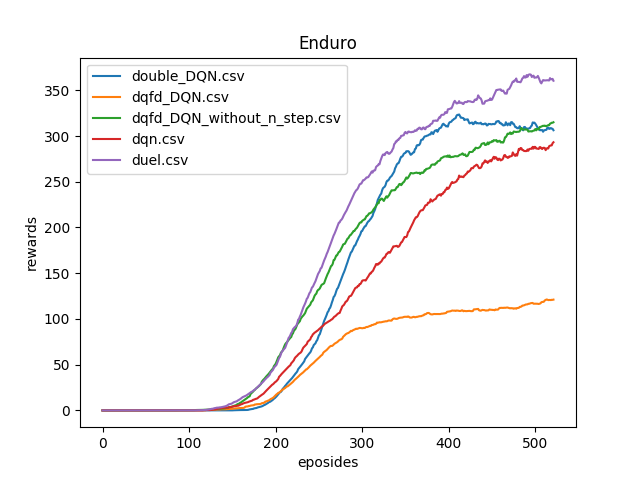
\includegraphics[width=0.15\textwidth]{Enduro}
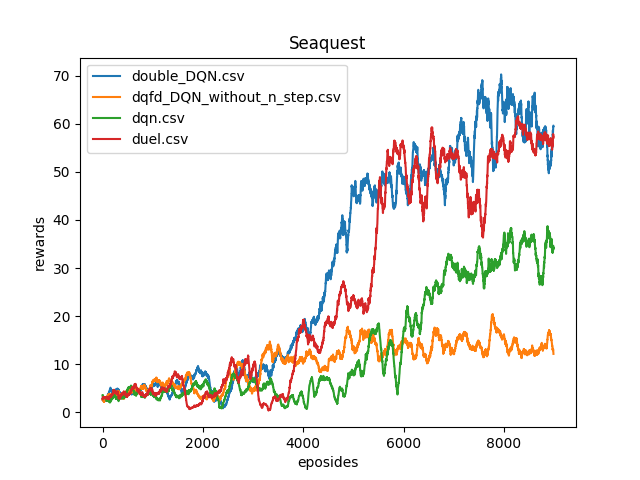
\includegraphics[width=0.15\textwidth]{Seaquest}
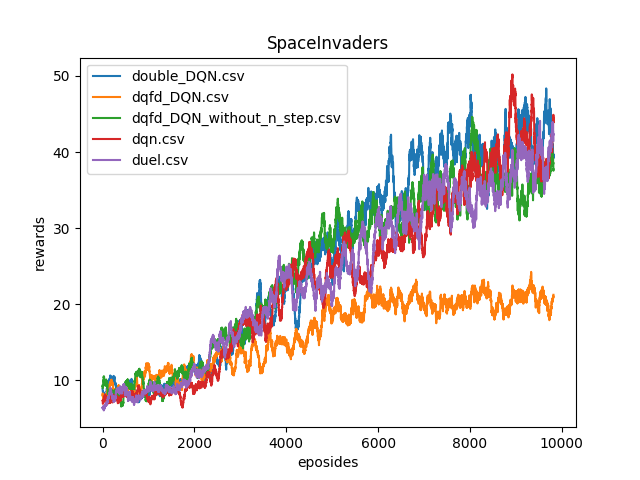
\includegraphics[width=0.15\textwidth]{SpaceInvaders}

We can see that DQfD didn't outperform other settings. Following is some of the reasons.

\begin{itemize}
\item We didn't implement Prioritized Experience Replay, and fix 30\% of batch size of data sampled from demonstration. This might be the reason why it didn't work.
\item According to the figure above, we can found n-step loss didn't help. There might be some implementation issues there.
\end{itemize}

 %----------------------------------------------------------------------------------------
%   REFERENCES
%----------------------------------------------------------------------------------------

\color{DarkSlateGray} % DarkSlateGray color for the rest of the content

\nocite{*} % Print all references regardless of whether they were cited in the poster or not
\bibliographystyle{plain} % Plain referencing style
\bibliography{poster} % Use the example bibliography file sample.bib


\end{multicols}
\end{document}
